For reference see figure \ref{fig:artemis}, equation \ref{eq:pid}, and table \ref{tab:myrio}. For citations use \cite{FSG}.

\begin{figure}[hbt!]
    \centering
    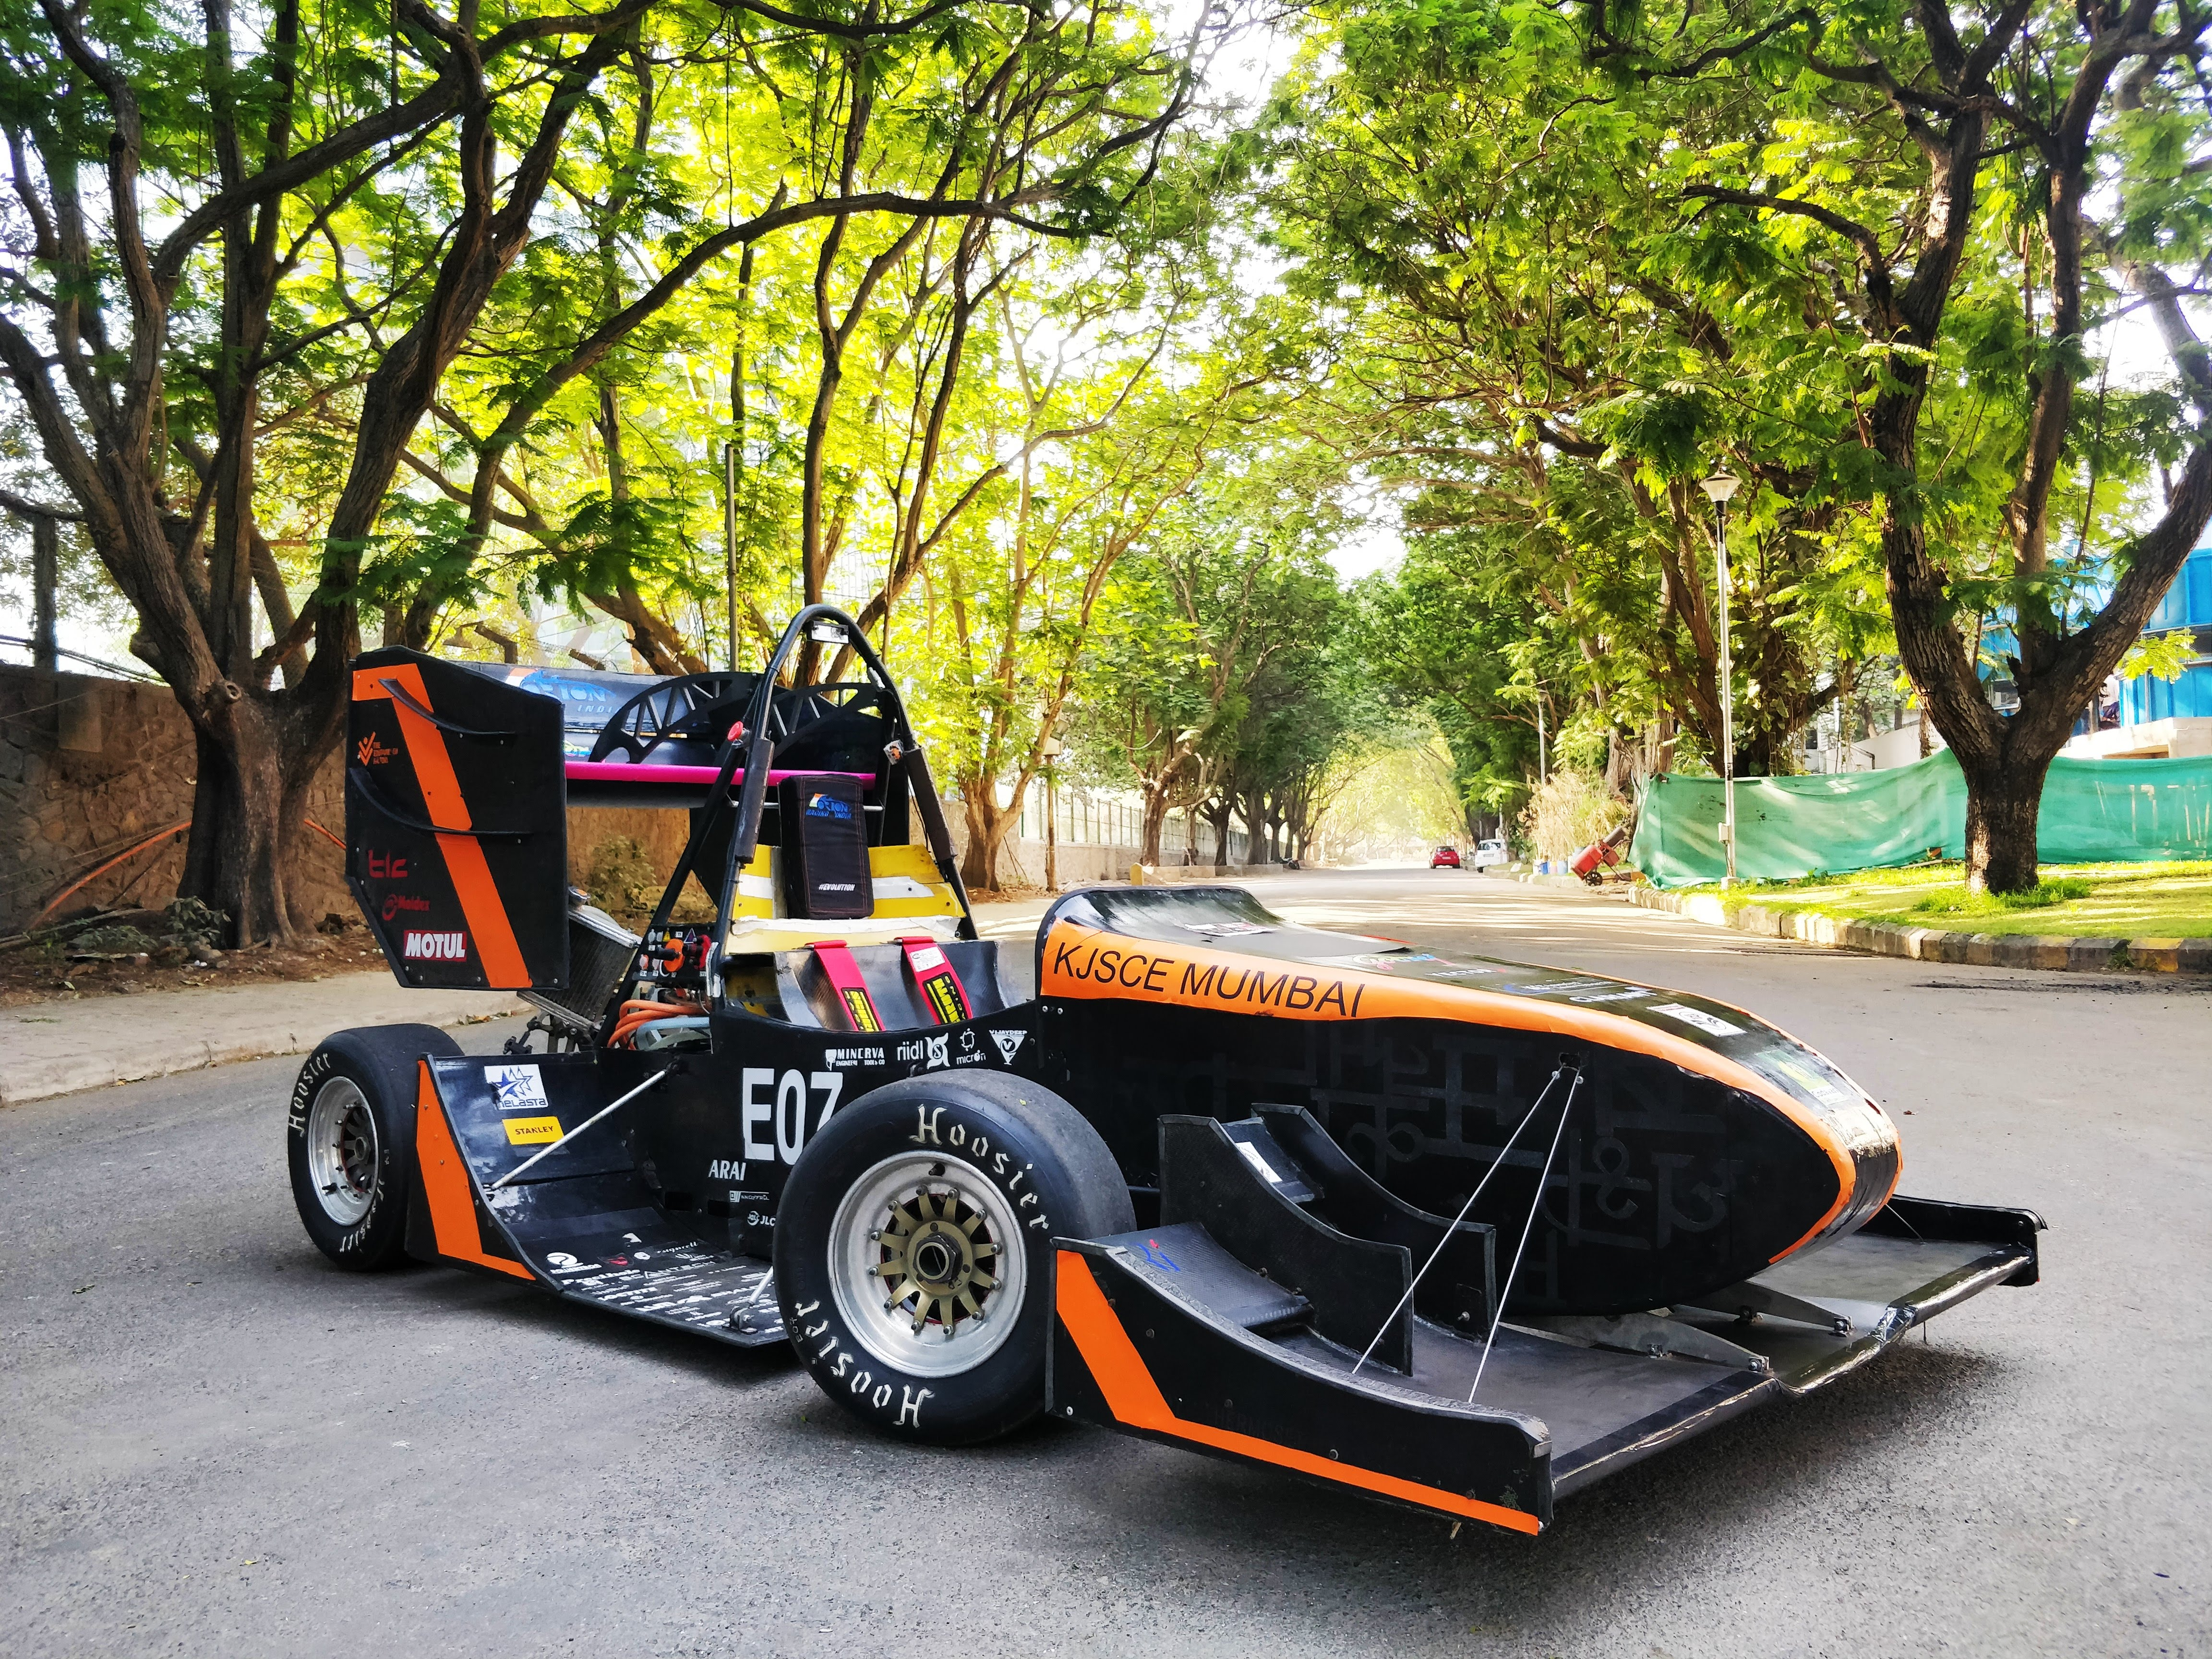
\includegraphics[width=0.8\textwidth]{images/Artemis.jpg}
    \caption{Artemis (ORI19e)}\label{fig:artemis}
\end{figure}

\[u(t) = K_p \ e(t) + K_i\ \int_{t_0}^{t} e(t') \ dt' + K_d \ \frac{de(t)}{dt}\] \label{eq:pid}

\begin{table}[hbt!]
\begin{center}
\scalebox{1}{%
\begin{tabular}{|M|L|}
 \hline
 \textbf{Components} & \textbf{Figures} \\
 \hline
 Processor & Xilinx FPGA and dual-core ARM Cortex-A9 processor \\ 
 \hline
 Max. Processor Operating Frequency & 667 MHz \\
 \hline
 Operating voltage & 6V - 16V \\
 \hline
 Program memory & 256 MB, DDR3 \\
 \hline
 Data memory & 512 MB, 533 MHz, 16 bits \\
 \hline
 Digital GPIOs & 40 \\
 \hline
 Analog pins & 10 (Input, 12-bit resolution), 6 (Output, 12-bit resolution) \\
 \hline
 Preferred programming language & LabVIEW \\
 \hline
 Max power consumption & 14 W \\
 \hline
 Wireless & IEEE 802.11/b/g/n ISM 2.4 GHz \\
 \hline
 USB & 2.0 Hi-Speed  \\
 \hline
 Inbuilt sensor & 3 axis accelerometer\\
 \hline
\end{tabular}}
\caption{\label{tab:myrio}NI myRIO important figures}
\end{center}
\end{table}
